\documentclass[12pt]{article}

\usepackage[top=50pt, bottom=50pt, left=90pt, right=90pt]{geometry}
\usepackage[pdftex]{graphicx}

\usepackage{lipsum}%% a garbage package you don't need except to create examples.
\usepackage{fancyhdr}
\pagestyle{fancy}

%This is some header and footer information
\lfoot{Kids Coding Club}
\rfoot{\thepage}
\cfoot{}
\renewcommand{\headrulewidth}{0pt}
\renewcommand{\footrulewidth}{0.4pt}

%Basic title information about original author and title
\title{Class 1 - Introduction to Coding}
\author{Chris Hight}
\date{\today}
 
 
%This is where we start the document
\begin{document}
\maketitle

\section*{Pre-Class Setup}
	\begin{itemize}
		
		\item Browser 1 - Private tabs
		\begin{itemize}
			\item Tab 1 - Scratch blank project
		\end{itemize}
		
		\item Browser 2
		\begin{itemize}
			\item Tab 1 - Red Light Green Light Project
		\end{itemize} 
		
		\item Slideshow for flow control

	\end{itemize}


\section*{Introduction}

\subsection*{Some Quick Talking Points}
	\begin{itemize}
		\item It’s ok to be frustrated when things don't work
		\begin{itemize}
			\item When something doesn't work and we need to fix it we call it debugging we will play a fun game with that in week 4
			\item Don’t give up on your code, start at the beginning of it and read through it.
			\item Sometimes it helps to have another coder look at it.
		\end{itemize}
	\end{itemize}


\subsection*{What is flow control}
	\begin{itemize}
		\item In Scratch it is called an "if then else" statement"
		\begin{itemize}
			\item This is a fork in the road for our code.  We are able to choose one direction or another based on a test for true or false statements.
			\item Red light green light game is flow control, E.G. \textbf{\textit{if}} the light is green \textbf{\textit{then}} we move, \textbf{\textit{else}} we stop
		\end{itemize}
		\item \textbf{show the control flow sideshow}
	\end{itemize}
	

\subsection*{Explain Boolean Values}
	\begin{itemize}
		\item Boolean values are true or false values. 
		\item Computers don't know the words true and false, Computers talk in 1’s and 0’s
		\item 1 = True
		\item 0 = False
		\item for us:
			\begin{itemize}
				\item 1 will equal true or that the light is green
				\item 0 will equal false or that the light is red
			\end{itemize}
	\end{itemize}


\subsection*{Example - Red Light, Green Light Game}
	\begin{itemize}
		\item We will need to add a background to our project. Click on add background and choose \textbf{track}
		\begin{center}
			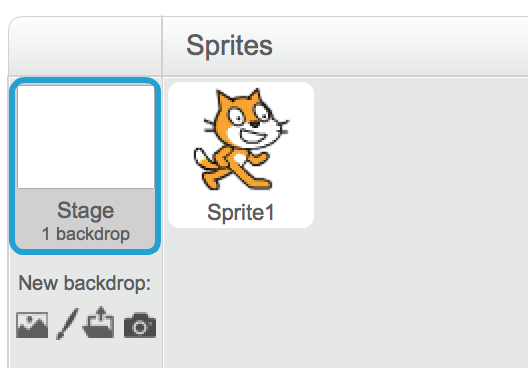
\includegraphics[scale=.50]{./Images/image1}
		\end{center}
		\item Next we need to add two sprites, \textbf{Stop} and \textbf{button4}
		\begin{center}
			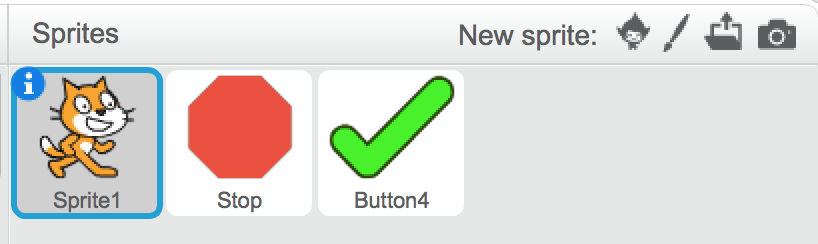
\includegraphics[scale=.50]{./Images/image2}
		\end{center}
		\item Drag the buttons so that our project looks like this
		\begin{center}
			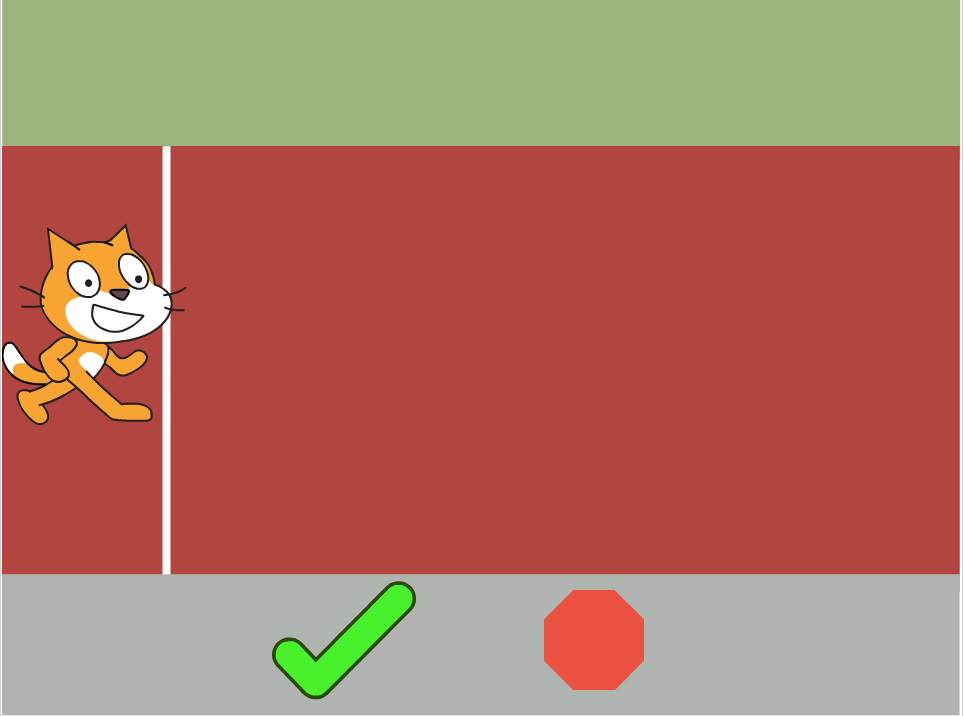
\includegraphics[scale=.50]{./Images/image3}
		\end{center}
		\item We need to build a data variable that our cat can read from, this will let him know if the light is green or red.  We will call it “GreenLight”
		\begin{center}
			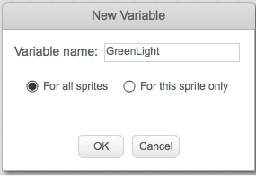
\includegraphics[scale=.50]{./Images/image4}
		\end{center}
		
		\item Lets make the variable GreenLight True when we click the check mark button
		\begin{itemize}
			\item In the check mark sprite, let's add a Event block that is when green flag clicked and a forever loop. 
			\item We want the program to check constantly that the button has been clicked
		\end{itemize}
		\begin{center}
			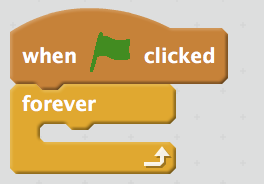
\includegraphics[scale=.8]{./Images/image5}
		\end{center}
		\item We are going to have an \textbf{if then} statement so that we can look for a click and when that happens we will set the variable.\begin{center}
			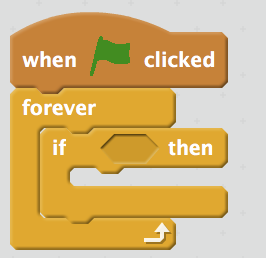
\includegraphics[scale=.8]{./Images/image6}
		\end{center}
		\item To recognize a button click we will need a couple of things, this will go into the if statement
			\begin{itemize}
				\item In the operators section we will need to use a logical “and” statement, this means next two things we add will both need to be true to enter the if statement
				\item First we will add a block from sensing called “touching” and we will set this to mouse-pointer.  This means that our pointer is touching the sprite
				\newpage
				\item Second we add a block from sensing called “mouse down?”.  This means that we have clicked the mouse button
			\end{itemize}
		\begin{center}
			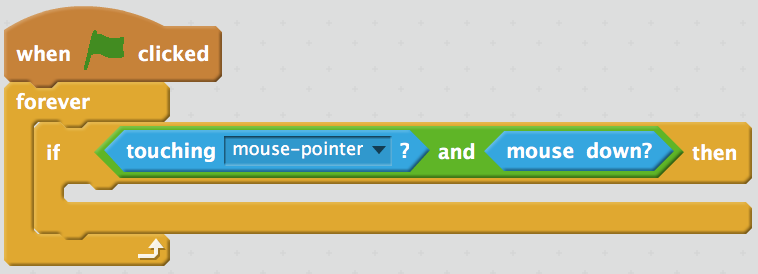
\includegraphics[scale=.6]{./Images/image7}
		\end{center}
		\item Inside the if statement we will set our green light variable.  Go to data and choose the “set” block.  Since this is the go button we want to set this to true which is “1”
		\begin{center}
			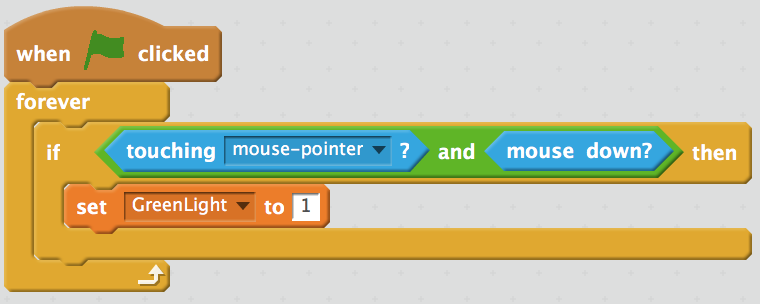
\includegraphics[scale=.6]{./Images/image8}
		\end{center}
		~\\~\\
		\item \textbf{\textit{***}}We will repeat the same thing for the stop button but we will set the variable to “0” for false
		\item Next we are going to set up our script for the cat to move. This will also involve a \textbf{if then} statement in which we will check if we have the green light to move
		\item We will start with the program start block from events
		\item we want to set the cat’s starting location, from the motion section we pick the “go to” block. I set this to -200 and 0
		\item Next we will use a forever block from the control section because we want the cat to be constantly checking to see if he should move
		\begin{center}
			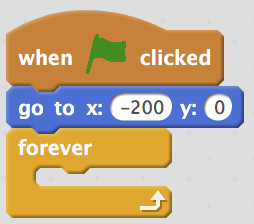
\includegraphics[scale=.8]{./Images/image9}
		\end{center}
		\item Add an \textbf{if then} statement to the inside of the forever statement so the cat can check and decide if he should move
		\item In operators we want to choose an equal statement because so that we can compare our variable to a green light
		\item Inside the equals block we want the first part to be the variable, from the data section we will drag the GreenLight variable
		\item In the second section we will enter the number 1
		\item Inside the if then statement we will add a block from motion called “move steps” that will make our character move.  enter the value 2
		\begin{center}
			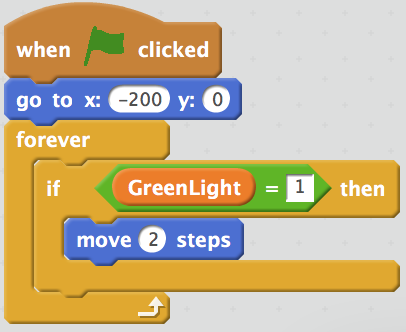
\includegraphics[scale=.8]{./Images/image10}
		\end{center}
	\end{itemize}

\end{document}